\documentclass[11pt,a4paper]{article}

\usepackage[margin=1in]{geometry}
\usepackage{amsmath,amssymb}
\usepackage{graphicx}
\usepackage{booktabs}
\usepackage{hyperref}
\usepackage{xcolor}
\usepackage{siunitx}

\title{Rate and Shape Information on the Higgs Self-Coupling in
$HH\to b\bar b\gamma\gamma$: A Detector-Level Phenomenological Study}

\author{Shreyansh Gupta}
\date{}

\begin{document}


\begin{abstract}
We study the dependence of Higgs-pair production on the Higgs self-coupling modifier $\kappa_\lambda$ in the $HH\to b\bar b\gamma\gamma$ final state at detector level. The analysis follows the information flow from the inclusive $gg\to HH$ production rate through event selection and reconstructed kinematic distributions. Five benchmark values, $\kappa_\lambda=\{-1.5,0,1,2,5\}$, are simulated at $\sqrt{s}=13$~TeV using MadGraph5\_aMC@NLO, Pythia 8, and Delphes. Forced Higgs decays are used to construct the $b\bar b\gamma\gamma$ final state, followed by a common detector-level selection.

We find a non-monotonic dependence of the production rate on $\kappa_\lambda$, while the detector-level selection efficiency also varies across the benchmark scan. The reconstructed $m_{HH}$ distribution retains substantial $\kappa_\lambda$ dependence, and the other reconstructed observables considered in this study exhibit corresponding shape variations. A descriptive pairwise shape-distance analysis is used to quantify these differences without interpreting them as statistical sensitivity. Finally, a signal-versus-signal boosted decision tree comparing $\kappa_\lambda=1$ and $\kappa_\lambda=2$ is studied. The resulting AUC of 0.565 is comparable to the AUC of 0.567 obtained using $m_{HH}$ alone, so no improvement from the multivariate combination is demonstrated within the present setup. The study provides a controlled detector-level characterization of rate and shape information while identifying the backgrounds, systematic uncertainties, larger simulated samples, and likelihood-based inference required for a quantitative determination of $\kappa_\lambda$.
\end{abstract}


The Higgs boson self-interaction is a central target of the Higgs physics program because it provides direct access to the structure of the electroweak symmetry-breaking potential. At hadron colliders, the trilinear Higgs coupling can be probed through Higgs-boson pair production, where the production amplitude contains both diagrams involving the Higgs self-coupling and diagrams that do not. Consequently, the dependence of the $HH$ production rate and kinematic distributions on the self-coupling parameter $\kappa_\lambda$ is intrinsically non-linear.

The non-resonant $HH\to b\bar b\gamma\gamma$ final state is particularly useful for phenomenological studies because it combines a sizeable branching fraction with a relatively clean diphoton signature. Previous studies have demonstrated sensitivity to the Higgs self-coupling through kinematic information, including the invariant mass of the Higgs-boson pair, and through multivariate techniques \cite{Goncalves2018,Alves2017}. More recent phenomenological studies have also investigated multivariate approaches to self-coupling measurements in this final state at higher-energy hadron colliders \cite{Park2020,Adhikary2020}. Experimentally, the $b\bar b\gamma\gamma$ channel has been used by ATLAS to constrain the Higgs self-coupling, including a recent analysis using 308~fb$^{-1}$ of data collected at 13 and 13.6~TeV \cite{ATLAS2025}.

In this work, we study the propagation of $\kappa_\lambda$-dependent information from the inclusive production rate to detector-level reconstructed observables in a controlled signal-only simulation of
\[
pp\to HH\to b\bar b\gamma\gamma.
\]
Rather than attempting to reproduce a complete experimental measurement, we separate three related aspects of the problem: the variation of the production rate, the variation of the selected signal yield after detector-level event selection, and the variation of normalized reconstructed kinematic shapes. We consider five benchmark values,
\[
\kappa_\lambda\in\{-1.5,0,1,2,5\},
\]
and study the reconstructed $m_{HH}$ distribution together with the transverse momenta and angular separations of the reconstructed Higgs candidates.

The analysis is designed as an information-flow study:
\[
\kappa_\lambda
\longrightarrow
\sigma_{HH}
\longrightarrow
\epsilon_{\rm sel}
\longrightarrow
N_{\rm sel}
\longrightarrow
\text{reconstructed shapes}.
\]
This allows the rate dependence and shape dependence to be discussed separately. We additionally perform a simple signal-versus-signal boosted decision tree (BDT) study to test whether combining several reconstructed observables improves discrimination between two representative self-coupling hypotheses relative to the $m_{HH}$ observable alone.

The study is intentionally limited in scope. It uses signal-only simulated samples and does not construct a complete background model, detector calibration model, systematic-uncertainty model, or experimental likelihood. Consequently, the results are not interpreted as an experimental exclusion interval or a projected measurement precision for $\kappa_\lambda$. Instead, the goal is to provide a transparent detector-level characterization of how self-coupling information appears in the rate and reconstructed shapes of the $b\bar b\gamma\gamma$ final state.


\section{Higgs-Pair Production and the Higgs Self-Coupling}

\subsection{\texorpdfstring{Dependence of $HH$ Production on $\kappa_\lambda$}{Dependence of HH Production on kappa-lambda}}

The Higgs self-coupling is parameterized in this work through the dimensionless modifier
$\kappa_\lambda$, defined by
\[
\lambda_{HHH}=\kappa_\lambda\,\lambda_{HHH}^{\rm SM},
\]
where $\lambda_{HHH}^{\rm SM}$ denotes the Standard Model trilinear Higgs coupling. The Standard Model point therefore corresponds to $\kappa_\lambda=1$.

At leading order, the dominant gluon-fusion contribution to non-resonant Higgs-pair production receives contributions from a box amplitude and a triangle amplitude. Schematically, the production amplitude can be written as
\[
\mathcal{M}_{gg\to HH}
=
\mathcal{M}_{\rm box}
+
\kappa_\lambda\,\mathcal{M}_{\rm triangle}.
\]
The corresponding cross section is therefore sensitive to both the magnitude of the self-coupling and its interference with the box contribution:
\[
\sigma_{HH}(\kappa_\lambda)
\propto
\left|
\mathcal{M}_{\rm box}
+
\kappa_\lambda\,\mathcal{M}_{\rm triangle}
\right|^2.
\]
This structure leads to a non-monotonic dependence of the production rate on $\kappa_\lambda$. In particular, changing $\kappa_\lambda$ does not simply rescale the Standard Model prediction; it also modifies the relative contribution and interference of the two production amplitudes. The resulting changes in the production kinematics can subsequently propagate into reconstructed detector-level observables \cite{Goncalves2018}.

In the present study we consider the benchmark set
\[
\kappa_\lambda=\{-1.5,0,1,2,5\}.
\]
The negative benchmark is treated as a phenomenological parameter point used to probe the dependence of the production amplitude on the sign and magnitude of the modified trilinear coupling. It is not interpreted as a statement about a physically realized negative Higgs self-coupling.

The benchmark scan is used consistently throughout the rate, detector-level shape, and multivariate analyses. This provides a common set of hypotheses with which to study how information on $\kappa_\lambda$ is transferred from the inclusive production process to the reconstructed $HH\to b\bar b\gamma\gamma$ final state.


\section{Event Generation and Detector-Level Analysis}

\subsection{Event Generation}

Signal events are generated for the non-resonant gluon-fusion process
\[
pp\to HH
\]
using MadGraph5\_aMC@NLO version 3.6.3. The loop-induced process is generated using the modified Standard Model UFO implementation with a variable Higgs trilinear coupling. The benchmark points considered are
\[
\kappa_\lambda=\{-1.5,0,1,2,5\}.
\]
The collider energy is $\sqrt{s}=13$~TeV. The NN23LO1 parton distribution function set is used together with the dynamical scale choice provided by the event-generation setup.

For the loop-induced production process, the matrix element is generated without a Born-level QCD contribution. The inclusive cross sections obtained from the event-generation scan are used as the normalization for the subsequent detector-level samples.

\subsection{Forced Higgs Decays}

The final state studied is
\[
HH\to b\bar b\gamma\gamma.
\]
Direct MadSpin decays were not used for the loop-induced Higgs-to-diphoton decay. Instead, the generated Higgs bosons were decayed with a dedicated two-body decay procedure that forces one Higgs boson to decay to $b\bar b$ and the other to $\gamma\gamma$ while preserving the original Higgs four-momentum.

The forced decay procedure was validated at generator level using the 10,000-event benchmark samples. The desired four-body final-state topology was obtained in 10,000/10,000 events, four-momentum conservation was satisfied in 10,000/10,000 events within numerical precision, and the reconstructed Higgs mass was consistent with the nominal value of approximately 125 GeV in 10,000/10,000 events. The two-body daughter systems also satisfied the expected back-to-back kinematic relation in 10,000/10,000 events. An additional check of the decay-angle distributions was statistically compatible with the expected isotropic two-body decay. These checks validate the generator-level forced-decay construction; they do not by themselves establish full detector-level equivalence to an independently simulated physical Higgs decay.

Because the forced-decay samples represent a specific decay topology, the physical $HH\to b\bar b\gamma\gamma$ branching fraction is restored when calculating expected event yields. We use
\[
{\rm BR}(H\to b\bar b)=0.5824,
\qquad
{\rm BR}(H\to\gamma\gamma)=0.00227,
\]
giving
\[
{\rm BR}(HH\to b\bar b\gamma\gamma)
=
2\,{\rm BR}(H\to b\bar b)\,
{\rm BR}(H\to\gamma\gamma)
=
0.0026441.
\]

\subsection{Parton Shower and Detector Simulation}

The generated events are passed to PYTHIA 8 for parton showering and hadronization and subsequently processed with DELPHES 3 using the ATLAS detector card. The detector simulation provides reconstructed jets, $b$-tagging information, and photons from which the analysis observables are constructed.

The detector-level study uses samples containing 10,000 generated events for each of the five benchmark values of $\kappa_\lambda$. These samples are used consistently for the cut-flow, reconstructed distributions, and pairwise shape comparisons.

The computational environment used for the analysis includes MadGraph5\_aMC@NLO 3.6.3, ROOT 6.32.24, and Python 3.10.12.

\subsection{Event Selection}

Jets are required to satisfy
\[
p_T^j>25~{\rm GeV},
\qquad
|\eta_j|<2.5,
\]
and events must contain at least two such jets. At least two of the selected jets must be $b$ tagged.

Photons are required to satisfy
\[
p_T^\gamma>25~{\rm GeV},
\qquad
|\eta_\gamma|<2.5,
\]
with at least two photons required in the event.

For events satisfying the object multiplicity requirements, the pair of $b$-tagged jets whose invariant mass is closest to the nominal Higgs-boson mass is chosen as the $H\to b\bar b$ candidate. The two leading photons are used to construct the diphoton candidate. The photon four-vectors are treated as massless when constructing the diphoton invariant mass.

The final signal selection requires
\[
100~{\rm GeV}<m_{bb}<150~{\rm GeV},
\]
and
\[
120~{\rm GeV}<m_{\gamma\gamma}<130~{\rm GeV}.
\]
The reconstructed Higgs-pair invariant mass is then calculated from the selected $b\bar b$ and $\gamma\gamma$ candidates:
\[
m_{HH}=m(b\bar b\gamma\gamma).
\]

The same selection is applied to all $\kappa_\lambda$ benchmark samples, allowing changes in the selected yield and reconstructed shapes to be compared without introducing benchmark-dependent selection requirements.


\section{Rate Information}

\subsection{Inclusive Production Rate}

The inclusive $HH$ production cross section exhibits the characteristic non-monotonic dependence on $\kappa_\lambda$ expected from the interference between the triangle and box amplitudes. For the benchmark points used in this study, the generated cross sections are
\[
\begin{array}{c|ccccc}
\kappa_\lambda & -1.5 & 0 & 1 & 2 & 5\\
\hline
\sigma_{HH}\;[\mathrm{pb}]
&0.070073&0.030540&0.014504&0.006786&0.033068
\end{array}
\]
with $\kappa_\lambda=1$ corresponding to the Standard Model benchmark.

The cross section reaches its smallest value among the considered benchmarks at $\kappa_\lambda=2$ and increases again towards $\kappa_\lambda=5$. This behavior illustrates why a measurement based only on the total rate can lead to non-trivial dependence on the assumed self-coupling parameter.

\subsection{Selection Efficiency}

The detector-level selection efficiency is defined as
\[
\epsilon_{\rm sel}
=
\frac{N_{\rm selected}}{N_{\rm generated}}.
\]
Each benchmark contains 10,000 generated signal events. The resulting efficiencies are
\[
\begin{array}{c|ccccc}
\kappa_\lambda & -1.5 & 0 & 1 & 2 & 5\\
\hline
\epsilon_{\rm sel}[\%]
&8.76&9.42&10.43&10.34&7.03
\end{array}
\]

The efficiency varies across the benchmark points, demonstrating that the detector-level selection does not act as a completely $\kappa_\lambda$-independent rescaling. The largest efficiency in the present benchmark set occurs at $\kappa_\lambda=1$, while the $\kappa_\lambda=5$ sample has the lowest efficiency.

The variation in efficiency is important when translating the inclusive production-rate dependence into a selected event yield. It also motivates treating rate and detector-level shape information as separate components of the analysis.

\subsection{Expected Selected Yield}

For the expected event yields, the physical branching fraction is restored according to
\[
{\rm BR}(HH\to b\bar b\gamma\gamma)=0.0026441.
\]
For an integrated luminosity $\mathcal{L}$ expressed in fb$^{-1}$, the selected signal yield is calculated as
\[
N_{\rm sel}
=
\sigma_{HH}\,[\mathrm{pb}]
\times
{\rm BR}(HH\to b\bar b\gamma\gamma)
\times
\epsilon_{\rm sel}
\times
\mathcal{L}\,[\mathrm{fb}^{-1}]
\times1000.
\]

At $\mathcal{L}=3000~\mathrm{fb}^{-1}$, the resulting selected signal yields are
\[
\begin{array}{c|ccccc}
\kappa_\lambda
&-1.5&0&1&2&5\\
\hline
N_{\rm sel}
&48.69&22.82&12.00&5.57&18.44
\end{array}
\]

Relative to the Standard Model benchmark, the corresponding selected yields are
\[
\begin{array}{c|ccccc}
\kappa_\lambda
&-1.5&0&1&2&5\\
\hline
N_{\rm sel}/N_{\rm SM}
&4.058&1.902&1.000&0.464&1.537
\end{array}
\]

Thus, in this signal-only detector-level study, the selected event rate varies substantially across the benchmark points. The yield dependence follows the inclusive cross-section dependence while also incorporating the benchmark-dependent selection efficiency.

Figure~\ref{fig:rate_summary} summarizes the inclusive cross section, detector-level selection efficiency, and expected selected yield as a function of $\kappa_\lambda$.

\begin{figure}[t]
    \centering
    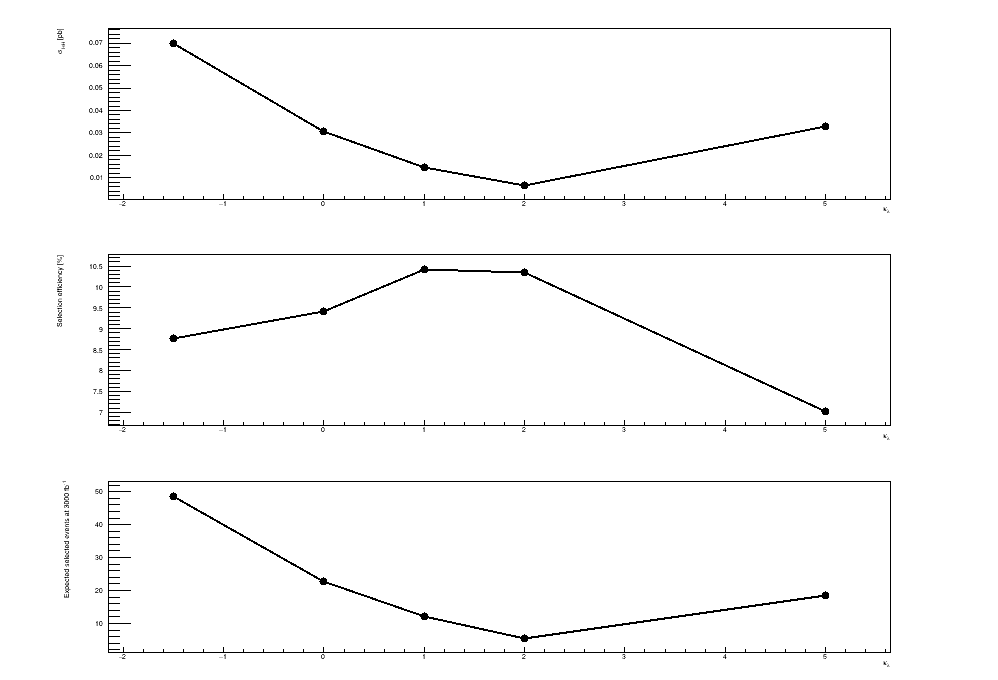
\includegraphics[width=\textwidth]{figures/rate_efficiency_yield_m15.png}
    \caption{Inclusive $HH$ production cross section, detector-level selection efficiency, and expected selected signal yield as functions of $\kappa_\lambda$. The expected yields assume an integrated luminosity of $3000~\mathrm{fb}^{-1}$ and include the physical $HH\to b\bar b\gamma\gamma$ branching fraction.}
    \label{fig:rate_summary}
\end{figure}


\section{Detector-Level Shape Information}

\subsection{\texorpdfstring{Reconstructed $m_{HH}$}{Reconstructed mHH}}

The reconstructed Higgs-pair invariant mass is one of the principal observables considered in this study because changes in $\kappa_\lambda$ modify the kinematics of the non-resonant $HH$ production process. After applying the common detector-level selection, the normalized $m_{HH}$ distributions are compared across the five benchmark points.

Figure~\ref{fig:mhh_shapes} shows the normalized reconstructed $m_{HH}$ distributions. The distributions exhibit benchmark-dependent shape variations in addition to the large rate differences discussed in the previous section. This demonstrates that the information carried by the selected sample is not restricted to the total event count.

The expected event distributions at $3000~\mathrm{fb}^{-1}$ are shown separately in Fig.~\ref{fig:mhh_expected}. In this representation, both the normalization and the shape dependence are visible. The large variation in normalization follows from the production cross section and selection efficiency, while differences in the normalized distributions isolate the shape component.

\begin{figure}[t]
    \centering
    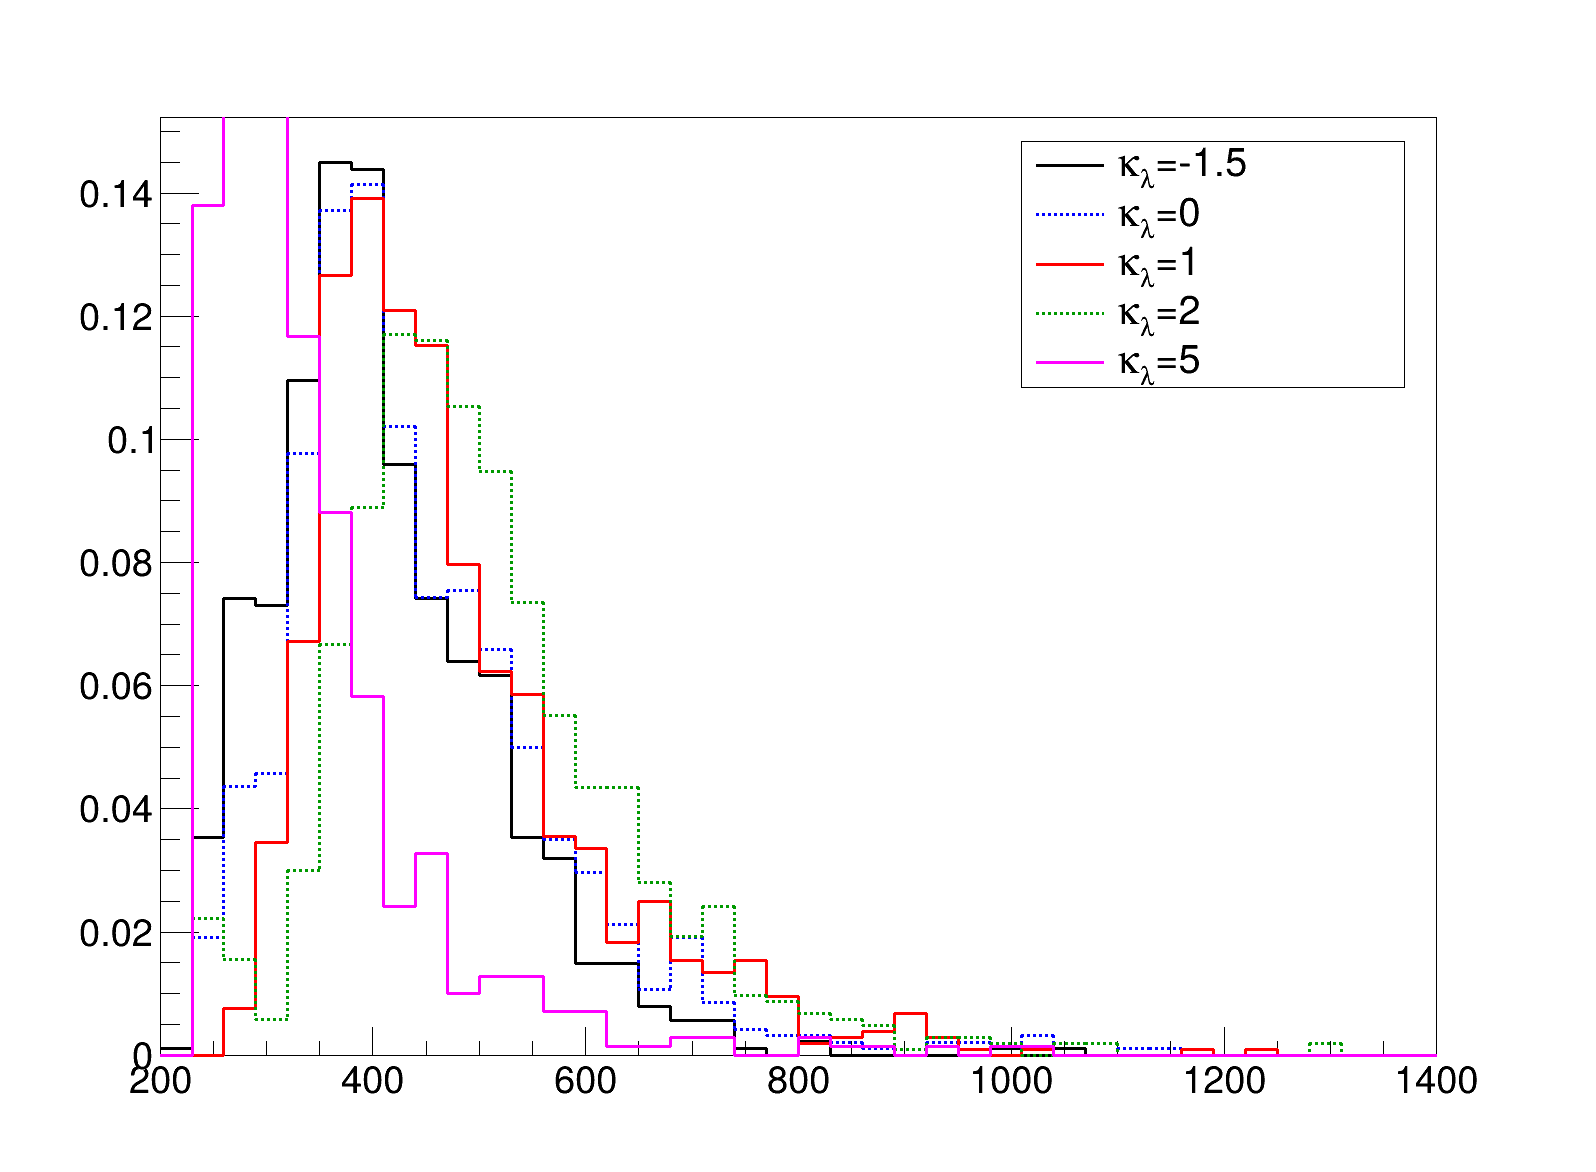
\includegraphics[width=0.82\textwidth]{figures/final_mhh_shapes_kl_m15.png}
    \caption{Normalized reconstructed $m_{HH}$ distributions after the common detector-level selection for the five benchmark values of $\kappa_\lambda$. The normalization of each distribution is independent of the total selected event yield, allowing the shape dependence to be examined separately from rate information.}
    \label{fig:mhh_shapes}
\end{figure}

\begin{figure}[t]
    \centering
    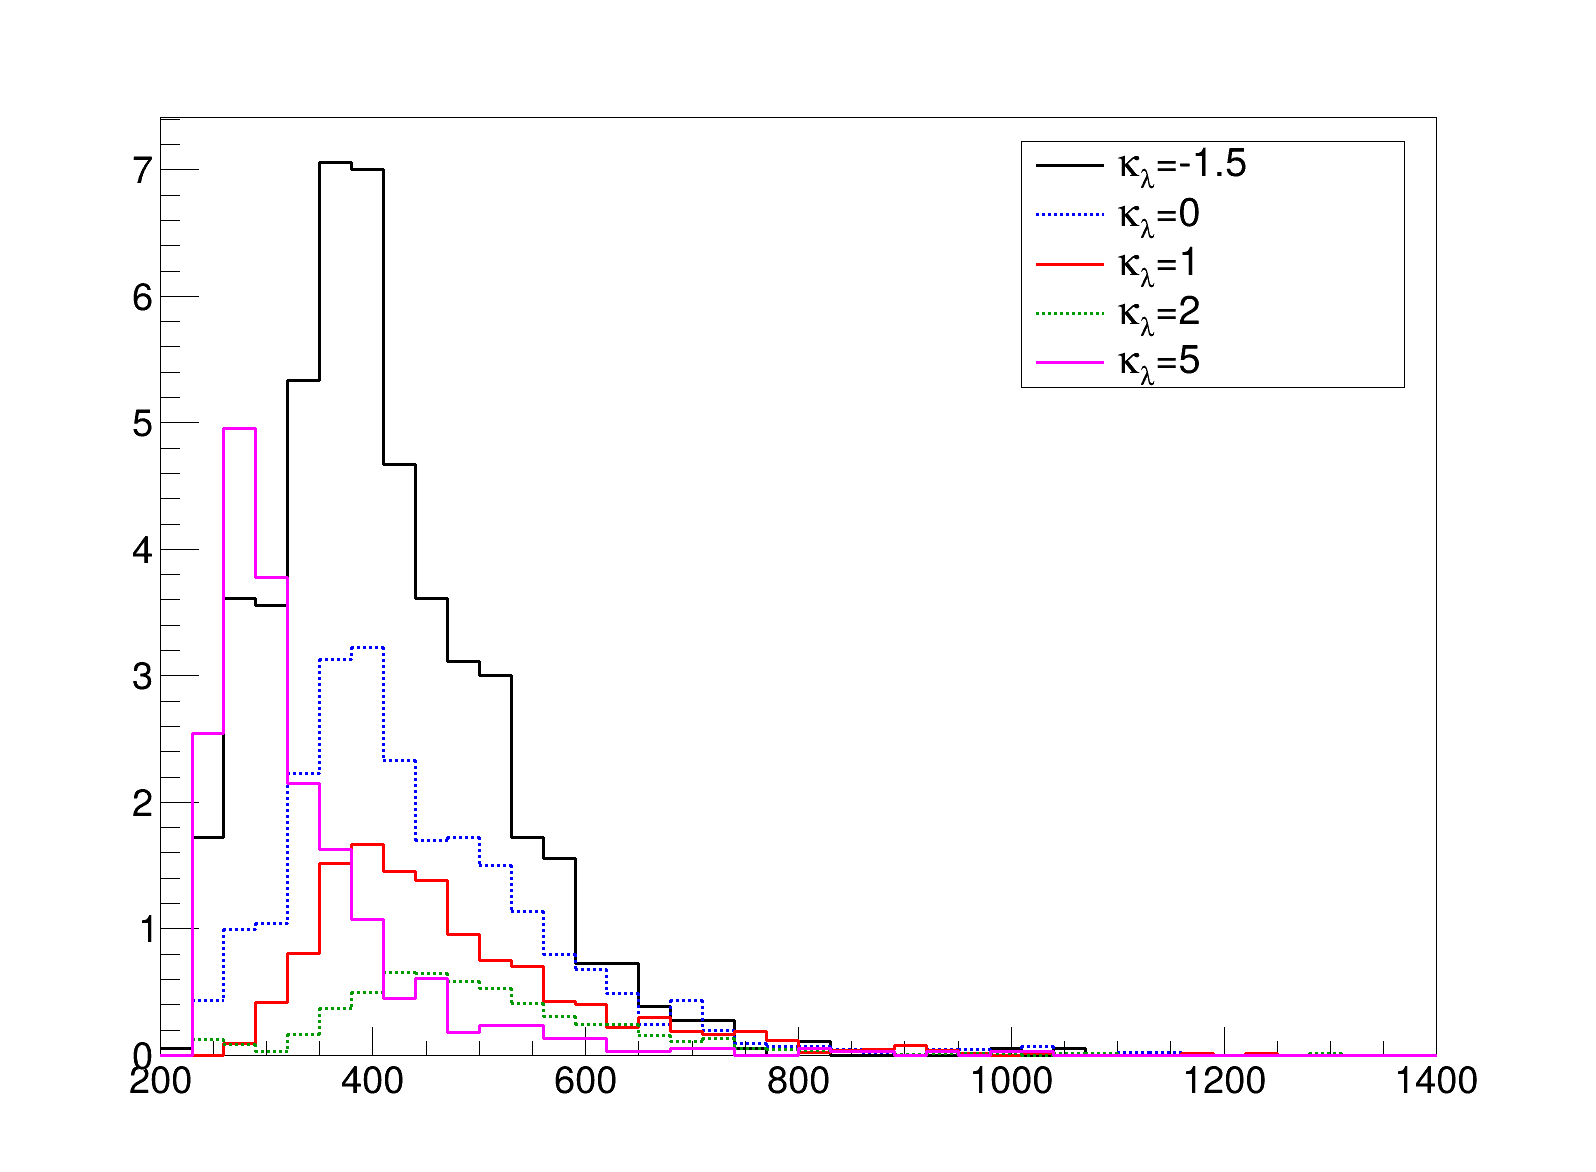
\includegraphics[width=0.82\textwidth]{figures/final_mhh_expected_kl_m15.png}
    \caption{Expected reconstructed $m_{HH}$ distributions for an integrated luminosity of $3000~\mathrm{fb}^{-1}$. Unlike the normalized distributions, these templates retain the benchmark-dependent signal normalization.}
    \label{fig:mhh_expected}
\end{figure}

\subsection{Other Reconstructed Observables}

To examine whether $\kappa_\lambda$ dependence is also visible in observables beyond $m_{HH}$, we also examine the reconstructed Higgs-candidate kinematics and angular variables. The observables considered are
\[
m_{bb},\quad
m_{\gamma\gamma},\quad
m_{HH},\quad
p_T(H_{bb}),\quad
p_T(H_{\gamma\gamma}),\quad
\Delta R_{bb},\quad
\Delta R_{\gamma\gamma}.
\]

The reconstructed Higgs-mass variables are primarily controlled by the event reconstruction and the mass-window selection. In contrast, the transverse-momentum and angular observables probe the event kinematics more directly and can therefore retain information about changes in the production dynamics.

The detector-level distributions for the seven observables are shown in Figs.~\ref{fig:scan_mbb}--\ref{fig:scan_drgg}. The same benchmark ordering and common selection are used throughout.

\begin{figure}[t]
    \centering
    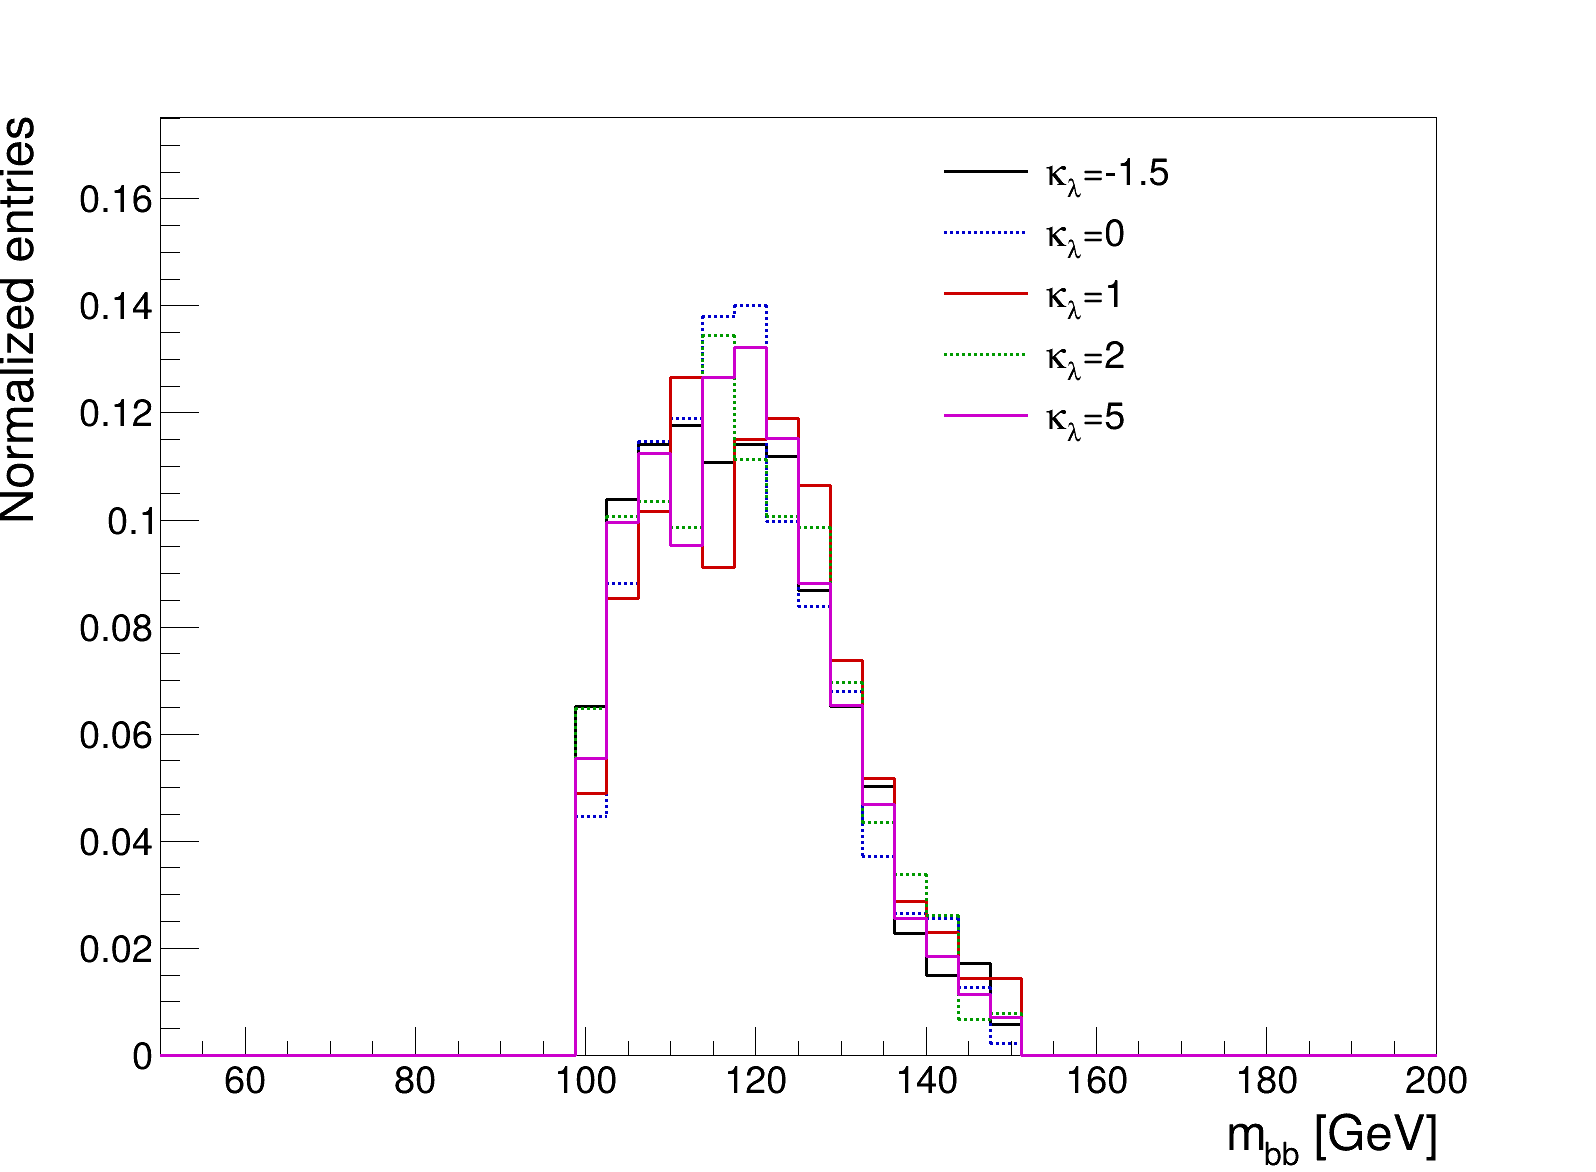
\includegraphics[width=0.82\textwidth]{figures/scan_mbb_kl.png}
    \caption{Reconstructed $m_{bb}$ distributions for the five $\kappa_\lambda$ benchmark points after the detector-level selection.}
    \label{fig:scan_mbb}
\end{figure}

\begin{figure}[t]
    \centering
    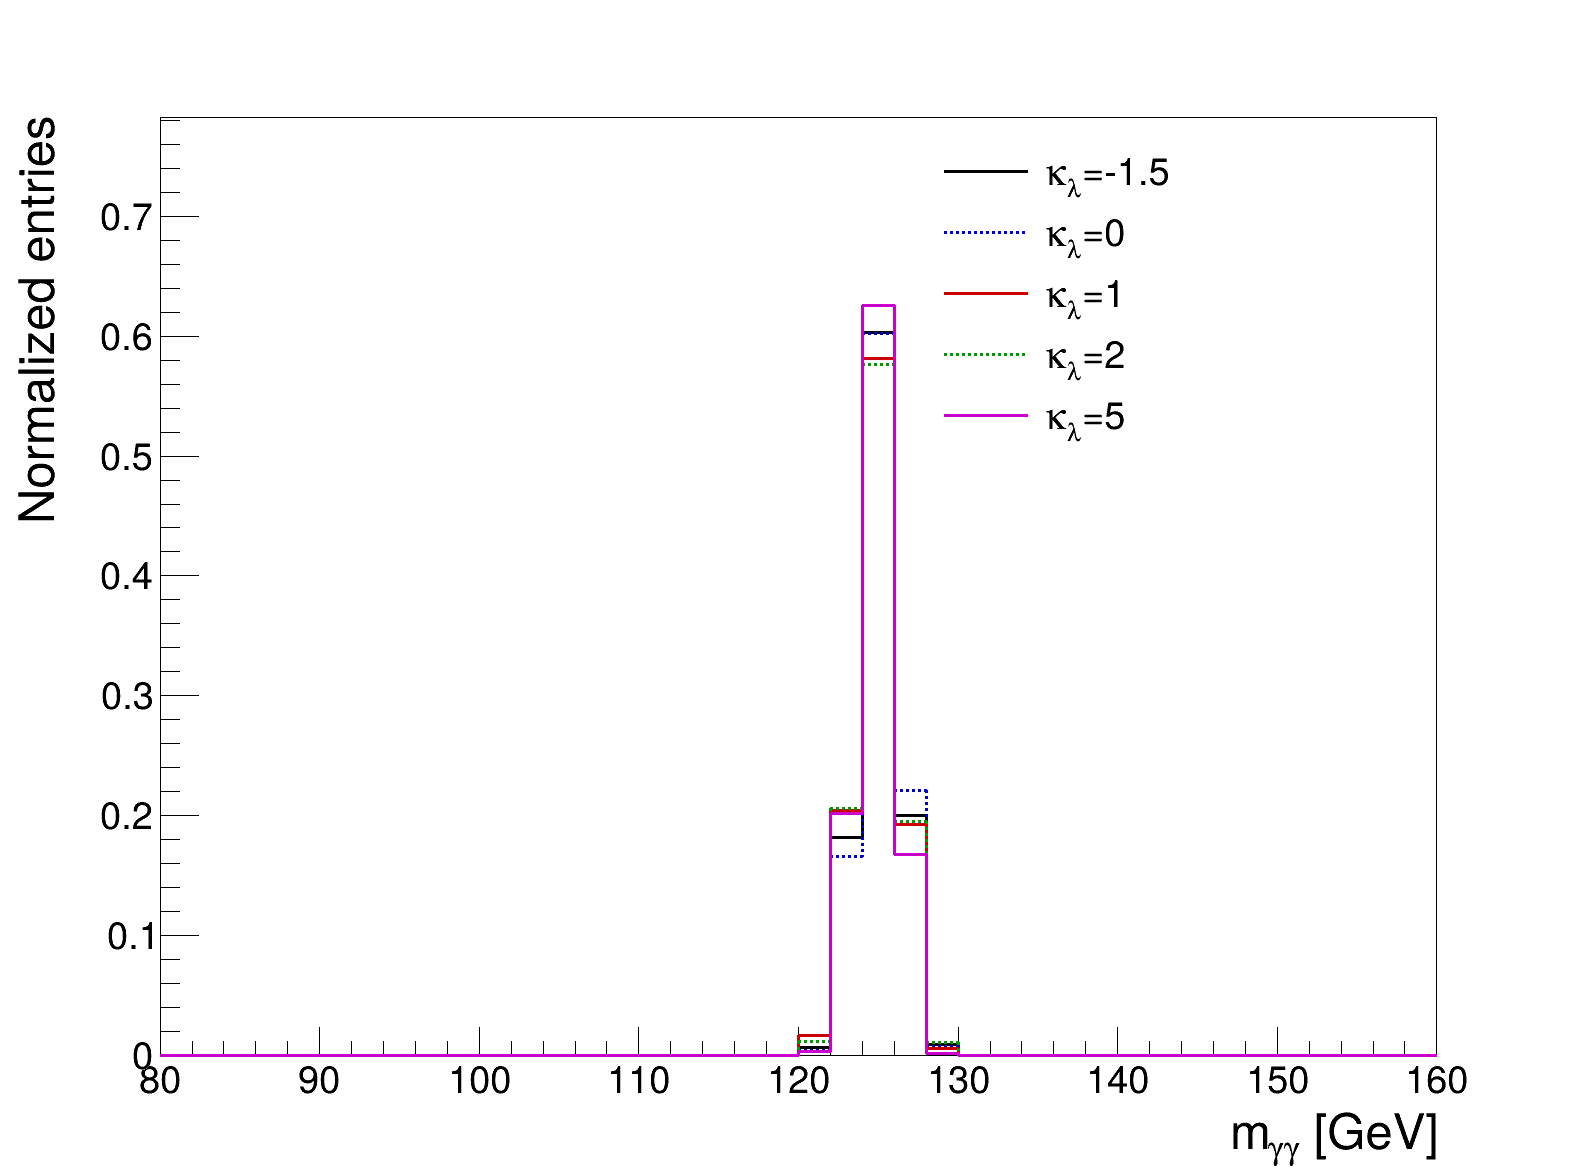
\includegraphics[width=0.82\textwidth]{figures/scan_mgg_kl.png}
    \caption{Reconstructed $m_{\gamma\gamma}$ distributions for the five $\kappa_\lambda$ benchmark points after the detector-level selection.}
    \label{fig:scan_mgg}
\end{figure}


\begin{figure}[t]
    \centering
    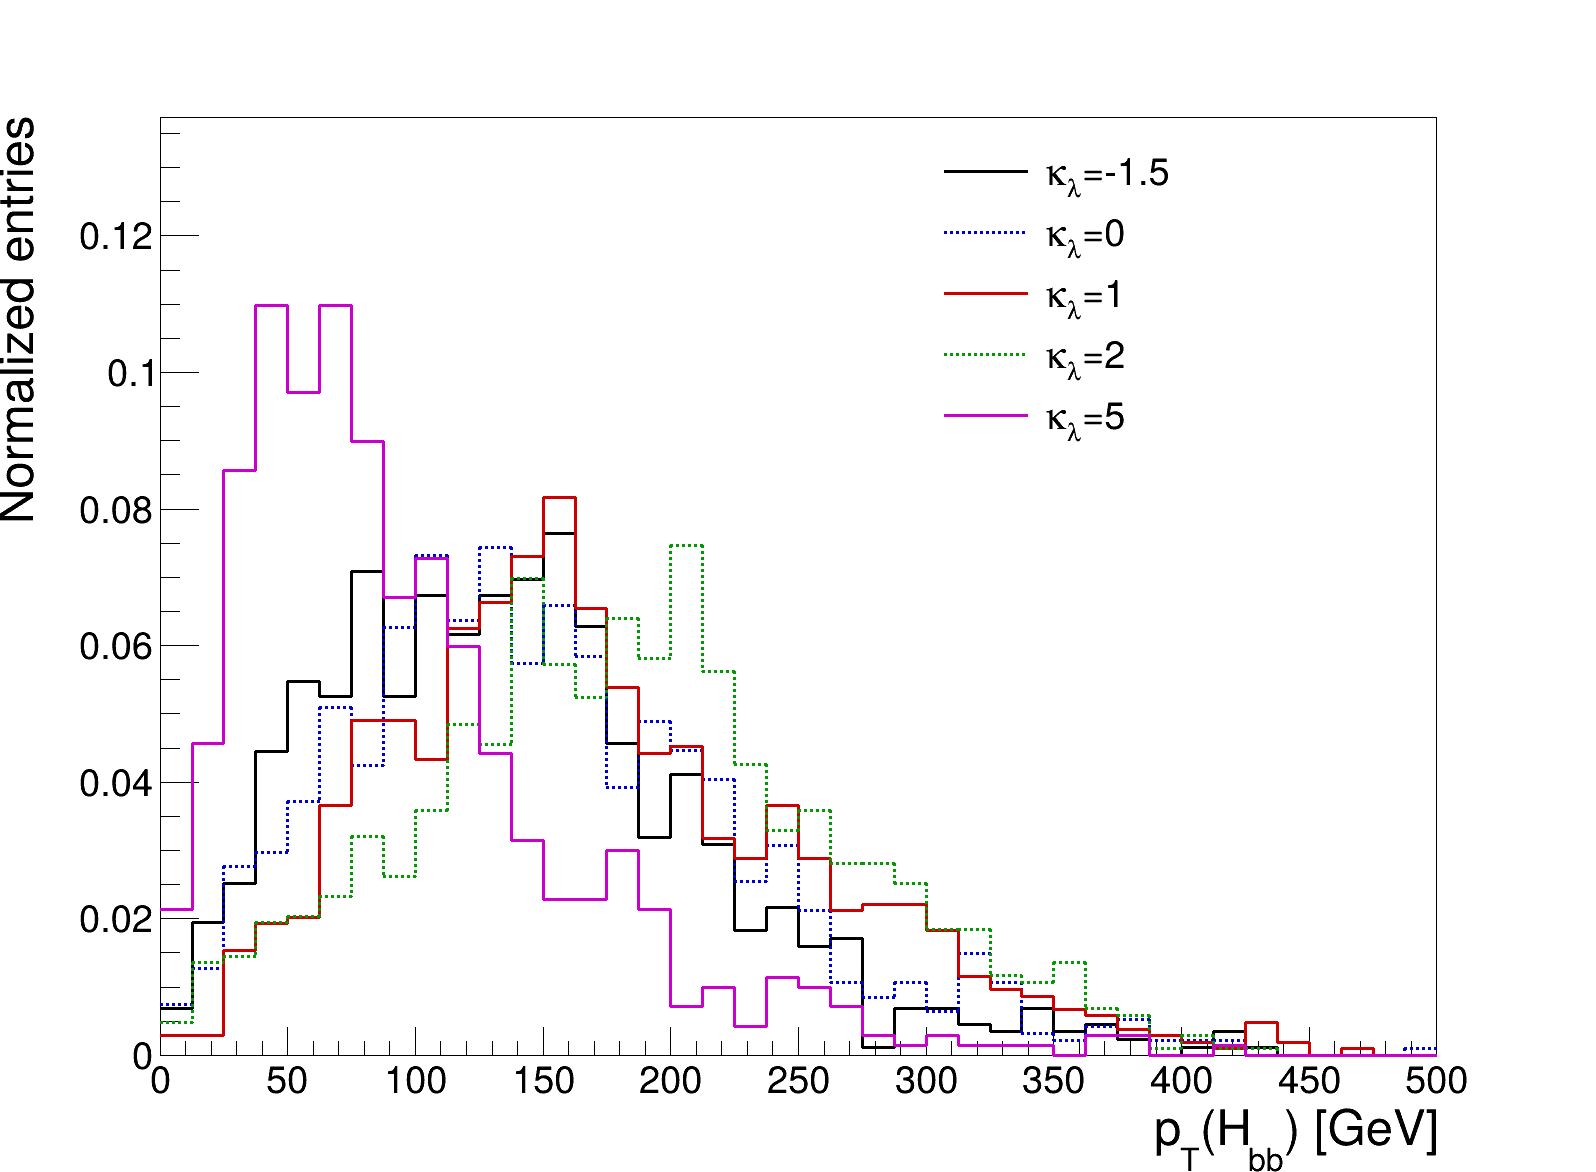
\includegraphics[width=0.82\textwidth]{figures/scan_ptbb_kl.png}
    \caption{Transverse momentum of the reconstructed $b\bar b$ Higgs candidate for the five $\kappa_\lambda$ benchmark points.}
    \label{fig:scan_ptbb}
\end{figure}

\begin{figure}[t]
    \centering
    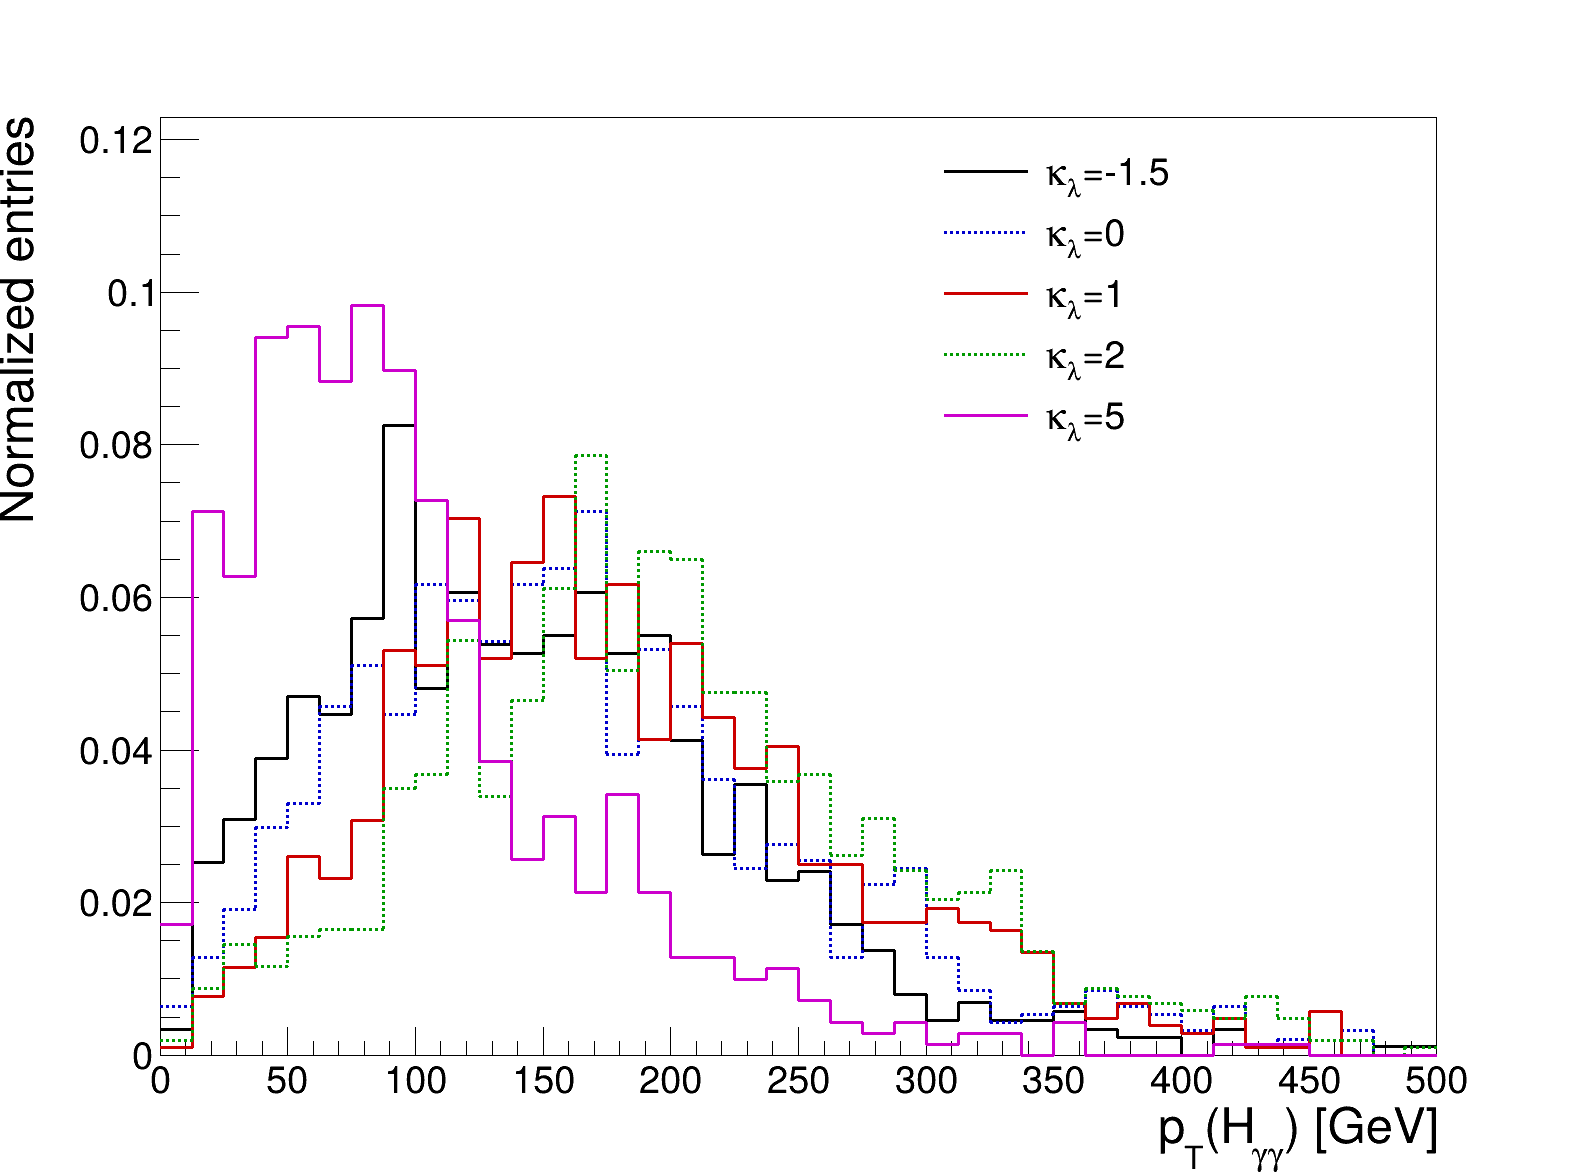
\includegraphics[width=0.82\textwidth]{figures/scan_ptgg_kl.png}
    \caption{Transverse momentum of the reconstructed $\gamma\gamma$ Higgs candidate for the five $\kappa_\lambda$ benchmark points.}
    \label{fig:scan_ptgg}
\end{figure}

\begin{figure}[t]
    \centering
    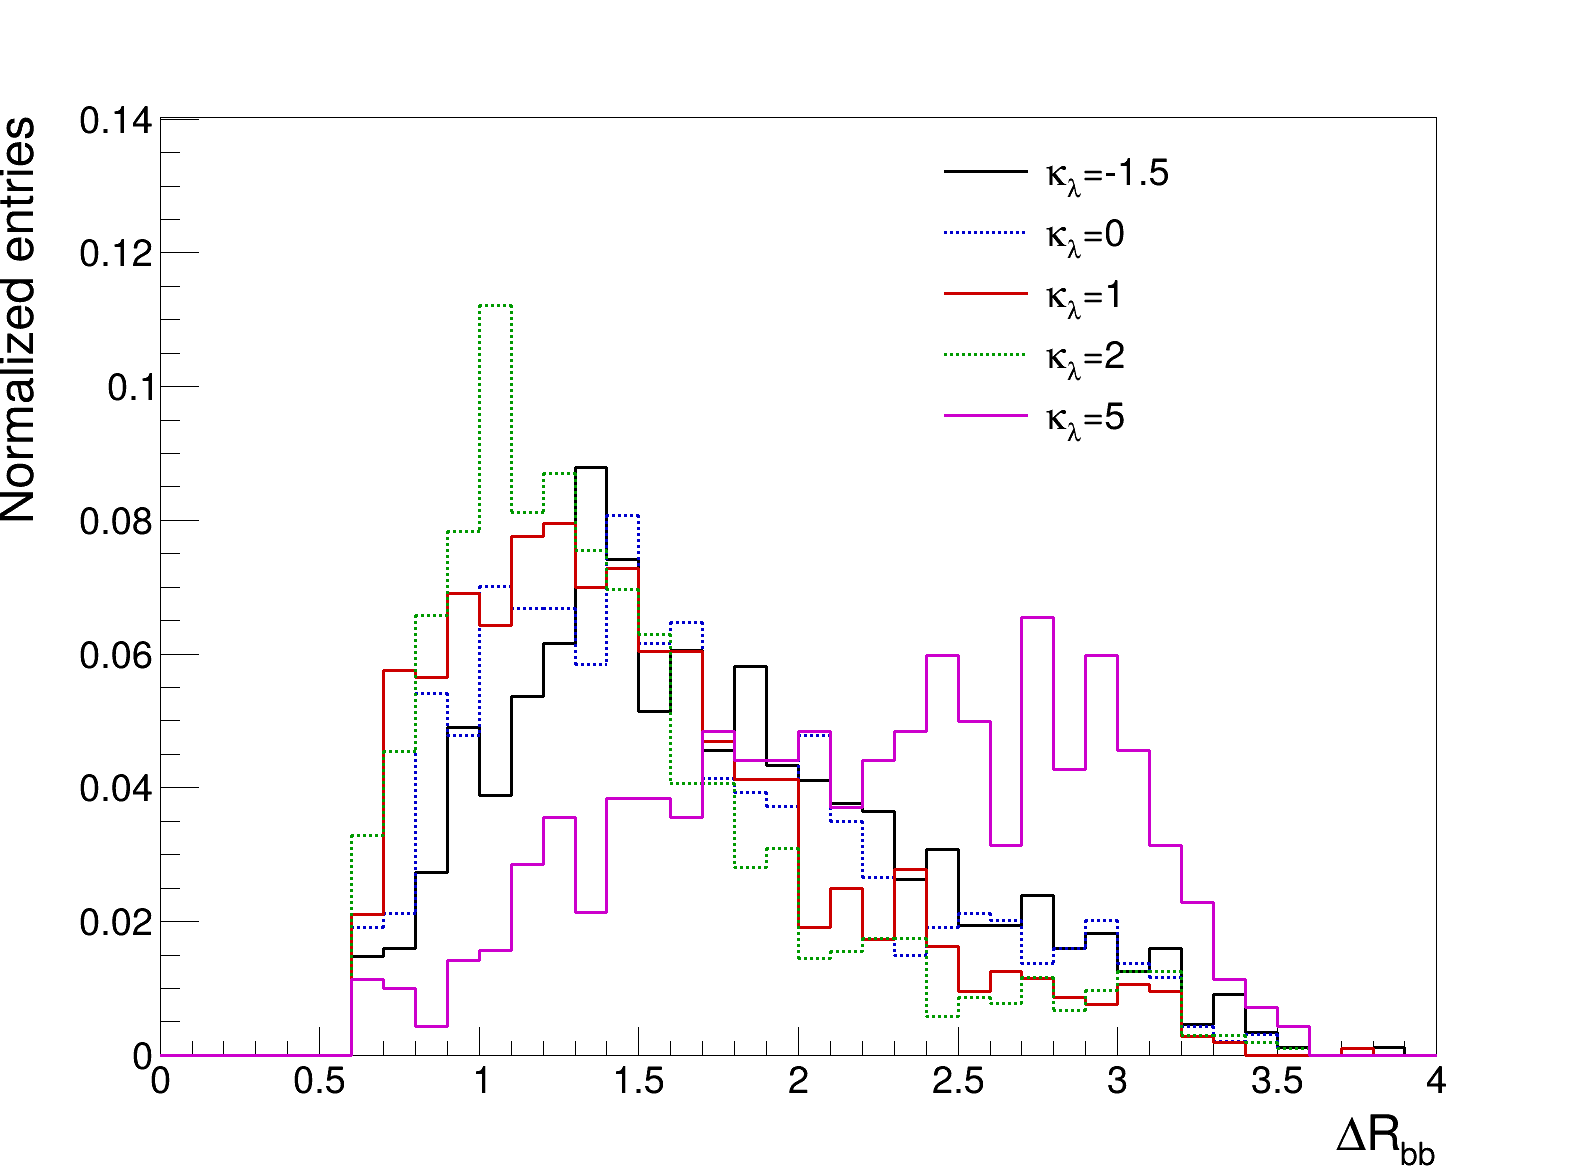
\includegraphics[width=0.82\textwidth]{figures/scan_drbb_kl.png}
    \caption{Angular separation $\Delta R_{bb}$ between the two selected $b$ jets for the five $\kappa_\lambda$ benchmark points.}
    \label{fig:scan_drbb}
\end{figure}

\begin{figure}[t]
    \centering
    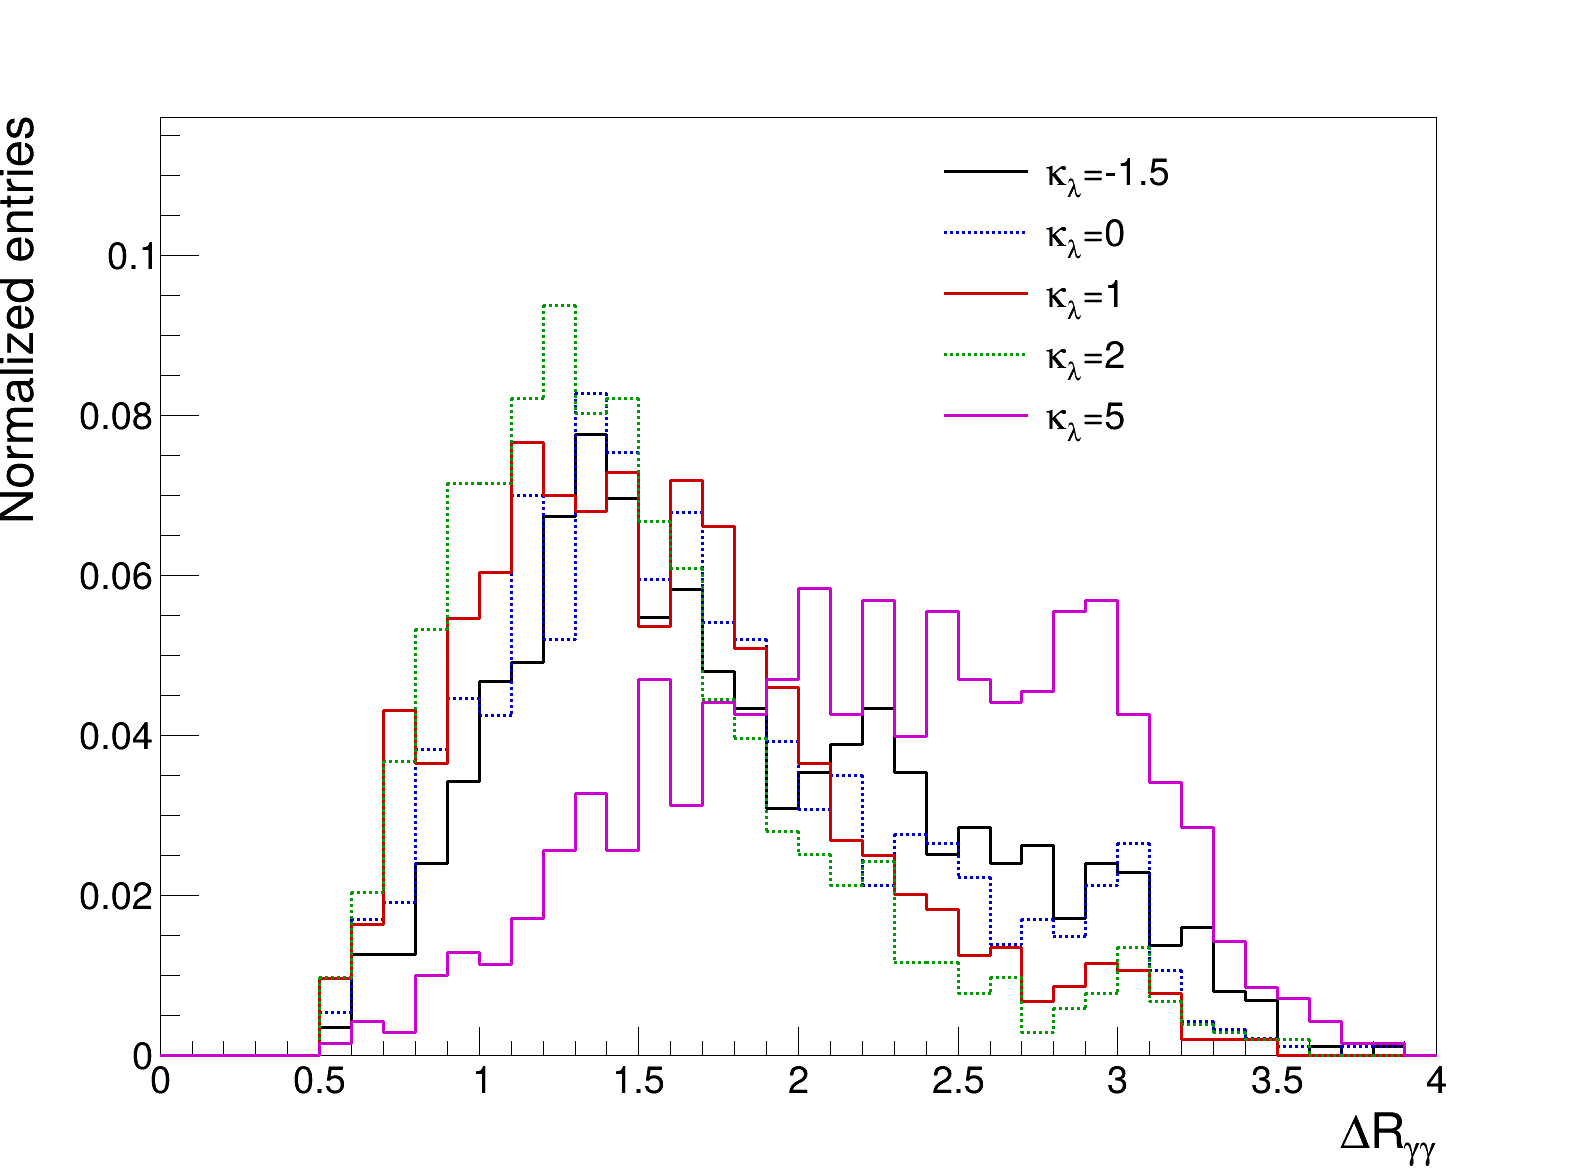
\includegraphics[width=0.82\textwidth]{figures/scan_drgg_kl.png}
    \caption{Angular separation $\Delta R_{\gamma\gamma}$ between the two selected photons for the five $\kappa_\lambda$ benchmark points.}
    \label{fig:scan_drgg}
\end{figure}

\subsection{Pairwise Shape-Distance Comparison}

To quantify the differences between normalized detector-level distributions, we define an exploratory pairwise shape-distance measure based on the normalized binned distributions. The resulting quantity is used only as a comparative diagnostic of shape differences between benchmark points. It is not interpreted as a likelihood ratio, statistical significance, or information-theoretic measure.

For each observable, all ten unique pairs among the five $\kappa_\lambda$ benchmarks are compared. The mean, minimum, and maximum distances are summarized in Table~\ref{tab:shape_distance}.

\begin{table}[t]
    \centering
    \caption{Summary of the exploratory pairwise shape-distance measure across the ten unique $\kappa_\lambda$ benchmark pairs.}
    \label{tab:shape_distance}
    \begin{tabular}{lccc}
        \toprule
        Observable & Mean & Minimum & Maximum \\
        \midrule
        $m_{bb}$ & 0.0099 & 0.0027 & 0.0165 \\
        $m_{\gamma\gamma}$ & 0.0030 & 0.0001 & 0.0100 \\
        $m_{HH}$ & 0.4277 & 0.0772 & 1.0569 \\
        $p_T(H_{bb})$ & 0.2527 & 0.0580 & 0.6434 \\
        $p_T(H_{\gamma\gamma})$ & 0.2521 & 0.0572 & 0.7023 \\
        $\Delta R_{bb}$ & 0.2181 & 0.0396 & 0.5928 \\
        $\Delta R_{\gamma\gamma}$ & 0.2150 & 0.0335 & 0.6201 \\
        \bottomrule
    \end{tabular}
\end{table}

Among the observables considered, $m_{HH}$ has the largest mean pairwise shape distance, while the transverse-momentum and angular observables also exhibit substantial benchmark dependence. The reconstructed Higgs-mass variables have considerably smaller shape distances, consistent with the fact that both are subject to explicit mass-window requirements in the event selection.

The $m_{HH}$ pairwise distances range from 0.0772 for the $\kappa_\lambda=-1.5$ versus $0$ comparison to 1.0569 for the $\kappa_\lambda=2$ versus $5$ comparison. Thus, the reconstructed $m_{HH}$ shape changes appreciably across the benchmark scan, although the magnitude of the change depends on the particular pair of hypotheses.

These comparisons establish that the detector-level dependence on $\kappa_\lambda$ contains a shape component in addition to the rate dependence. The shape-distance analysis is intentionally used as a descriptive comparison; a quantitative determination of experimental sensitivity would require a statistical model including backgrounds, uncertainties, and correlations among observables.


\section{Multivariate Study}

\subsection{BDT Setup}

To investigate whether combining several reconstructed observables provides additional discrimination between different values of $\kappa_\lambda$, a boosted decision tree (BDT) study was performed. The analysis was formulated as a signal-versus-signal classification problem between the $\kappa_\lambda=1$ and $\kappa_\lambda=2$ benchmark samples. This choice provides a controlled test of whether detector-level kinematic information can distinguish two different self-coupling hypotheses without introducing a background-classification problem.

The BDT used four reconstructed observables:
\begin{equation}
\left\{m_{HH},\;p_T(H_{bb}),\;p_T(H_{\gamma\gamma}),\;\Delta R_{bb}\right\}.
\end{equation}
The $\kappa_\lambda=2$ sample contained 1622 selected events, of which 1135 were used for training and 487 for testing. The classifier was configured with 50 trees, a maximum tree depth of 2, a minimum node size of 15\%, AdaBoost with $\beta=0.5$, the Gini separation criterion, and 20 cut points.

The resulting test-sample area under the receiver-operating-characteristic curve (AUC) was 0.565. The RMS variation of the AUC over 20 training/test splits was 0.018. The relatively modest AUC indicates that the two signal hypotheses are only weakly separated by the selected set of reconstructed observables in this analysis.

\subsection{\texorpdfstring{Comparison with $m_{HH}$}{Comparison with mHH}}

To assess whether the multivariate combination provides information beyond the principal reconstructed observable, the BDT result was compared with one-dimensional classifiers constructed from each input variable separately. The corresponding AUC values were
\begin{equation}
\begin{array}{c|c}
\text{Observable} & \text{AUC} \\
\hline
m_{HH} & 0.567 \\
p_T(H_{bb}) & 0.537 \\
p_T(H_{\gamma\gamma}) & 0.543 \\
\Delta R_{bb} & 0.525 \\
\text{BDT combination} & 0.565
\end{array}
\end{equation}

In this signal-versus-signal test, the BDT combination does not show a clear improvement over $m_{HH}$ alone. The $m_{HH}$ classifier gives an AUC of 0.567, compared with 0.565 for the four-variable BDT. This result should not be interpreted as evidence that the additional observables contain no information about $\kappa_\lambda$. Rather, within the present detector-level sample size, feature set, and simple BDT configuration, their combination does not produce a measurable improvement over $m_{HH}$ for the particular $\kappa_\lambda=1$ versus $\kappa_\lambda=2$ comparison.

The multivariate result therefore serves primarily as a consistency check on the shape analysis. It demonstrates that the presence of $\kappa_\lambda$-dependent differences in several reconstructed observables does not automatically imply an improved multivariate separation. A more quantitative assessment would require larger simulated samples, systematic variations, background processes, and a statistical inference framework.

\section{Discussion and Limitations}

The results provide a consistent detector-level picture of how information on the Higgs self-coupling is propagated through the $HH\to b\bar b\gamma\gamma$ analysis chain. At the production level, the $HH$ cross section varies non-monotonically with $\kappa_\lambda$, reflecting the interference between the box and triangle contributions to the $gg\to HH$ amplitude. After detector simulation and event selection, the selected-event efficiency also varies across the benchmark points, ranging from 7.03\% for $\kappa_\lambda=5$ to 10.43\% for $\kappa_\lambda=1$. Consequently, the expected selected event yield contains information from both the production rate and the selection efficiency.

The reconstructed distributions additionally retain $\kappa_\lambda$ dependence after detector-level selection. Among the observables considered, $m_{HH}$ exhibits the largest mean pairwise shape distance according to the descriptive metric used in this study. The other reconstructed quantities, including $p_T(H_{bb})$, $p_T(H_{\gamma\gamma})$, $\Delta R_{bb}$, and $\Delta R_{\gamma\gamma}$, also show benchmark-dependent shape variations. These observations support the interpretation that the detector-level information is not limited to the inclusive event rate.

The multivariate study provides a complementary result. For the $\kappa_\lambda=1$ versus $\kappa_\lambda=2$ signal-versus-signal classification, the four-variable BDT gives an AUC of 0.565, compared with 0.567 for $m_{HH}$ alone. Within the present setup, therefore, the combination of the selected observables does not demonstrate an improvement over the principal one-dimensional observable. This result is useful as a consistency check: differences in several distributions do not necessarily translate into improved multivariate separation for a particular pair of hypotheses and a finite simulated sample.

Several limitations should be emphasized. First, the analysis is signal-only and does not include continuum or resonant background processes. The reported AUC values therefore describe separation between two signal hypotheses rather than signal-versus-background performance. Second, no detector calibration, experimental systematic uncertainties, theoretical uncertainties, or correlations between systematic nuisance parameters are included. Third, the study uses fast detector simulation with the Delphes ATLAS detector card rather than a full detector simulation. The forced Higgs decays used to obtain the $b\bar b\gamma\gamma$ final state were validated at generator level, but this validation does not establish equivalence to a fully simulated natural Higgs decay treatment.

The simulated samples contain 10,000 generated events for each benchmark point. The resulting selected samples are therefore suitable for a controlled phenomenological comparison, but they are not sufficient for a precision sensitivity study. In particular, the shape-distance quantities are descriptive measures of differences between normalized distributions and should not be interpreted as likelihood ratios, statistical significances, Fisher information, or projected confidence intervals.

Finally, the present analysis does not perform a statistical inference of $\kappa_\lambda$. No likelihood fit, confidence interval, exclusion limit, or projected experimental precision is derived. The purpose is instead to separate and illustrate three stages of information: the $\kappa_\lambda$ dependence of the inclusive production rate, the modification introduced by detector-level selection and reconstructed shapes, and the extent to which a simple multivariate combination captures additional separation beyond $m_{HH}$. A future sensitivity study could extend this framework by incorporating backgrounds, larger simulated samples, systematic uncertainties, correlated observables, and a dedicated likelihood-based statistical analysis.

\section{Conclusions}

This study investigated how information on the Higgs self-coupling parameter $\kappa_\lambda$ is transferred from the inclusive $HH$ production rate to detector-level observables in the $HH\to b\bar b\gamma\gamma$ final state. Five benchmark hypotheses, $\kappa_\lambda=\{-1.5,0,1,2,5\}$, were studied using loop-induced $gg\to HH$ event generation, forced Higgs decays, Pythia 8 showering, and Delphes detector simulation.

The inclusive production rate shows the expected non-monotonic dependence on $\kappa_\lambda$ arising from interference between the box and triangle amplitudes. After detector-level selection, the efficiency varies across the benchmark points, so the selected event yield contains both production-rate and selection-efficiency dependence. At an illustrative luminosity of $3000~\mathrm{fb}^{-1}$, the expected selected yields range from approximately 5.57 events for $\kappa_\lambda=2$ to 48.69 events for $\kappa_\lambda=-1.5$, before any background contribution or statistical inference is considered.

The reconstructed observables retain additional $\kappa_\lambda$ dependence after selection. In particular, the $m_{HH}$ distribution exhibits substantial shape variation across the benchmark scan, with the descriptive pairwise shape-distance measure ranging from 0.0772 to 1.0569. Other reconstructed observables, including Higgs transverse momenta and angular separations, also exhibit benchmark-dependent shape differences. These results demonstrate that the detector-level dependence on $\kappa_\lambda$ is not represented solely by the inclusive production rate.

A signal-versus-signal BDT study was used as a complementary test of whether combining several observables produces additional separation. For the $\kappa_\lambda=1$ versus $\kappa_\lambda=2$ comparison, the four-variable BDT achieved an AUC of 0.565, while $m_{HH}$ alone gave an AUC of 0.567. Within the present sample size, feature set, and classifier configuration, the multivariate combination therefore did not demonstrate an improvement over $m_{HH}$ alone.

Overall, the analysis provides a controlled detector-level information-flow study of Higgs self-coupling dependence in the $HH\to b\bar b\gamma\gamma$ channel. It separates the contributions of production rate, selection efficiency, reconstructed shape information, and a simple multivariate combination, while avoiding claims of experimental sensitivity or statistical inference. Extending this framework to a quantitative determination of $\kappa_\lambda$ would require larger simulated samples, backgrounds, systematic uncertainties, correlated observables, and a likelihood-based statistical analysis.

\bibliographystyle{unsrt}
\bibliography{references}

\end{document}
